\chapter{About the evaluated tools}
\label{chap:tools}

In this chapter, the evaluated tools are described in more detail together with information about how they are used to implement the proof-of-concept application.

\section{Apache Cordova}

\subsection{General information \& history}

Apache Cordova\footnote{\url{http://cordova.apache.org}} started out as a project called PhoneGap. It was developed by a couple of employees from a Canadian company called Nitobi and was unofficially released at the iPhoneDevCamp gathering in August 2008. In 2011, Adobe acquired the company such that the team could focus solely on the development of PhoneGap. At the same time, Nitobi donated the PhoneGap codebase to the Apache Software Foundation (ASF), where it became an incubating\footnote{In order to become part of the ASF, every project is required to go through an incubating stage.} project. To make sure that the intellectual property would not conflict with trademark ambiguity, the project's name was changed from PhoneGap to Apache Callback. Because the community was dissatisfied with the project's name, it was quickly changed to Apache Cordova. On October 2012, Apache Cordova graduated as a top level project within the Apache Software Foundation. This ensures that it will always remain free and open source under the Apache License 2.0.

Nowadays, PhoneGap is a distribution of Apache Cordova, delivered by Adobe. PhoneGap strategically fits in a collection of software like Adobe PhoneGap Build and Adobe Edge Inspect. The development and maintenance of the cross-platform tool happens in the Apache Cordova project and is driven by an active community in which Adobe is the largest contributor.

Apache Cordova supports a large number of platforms, both mobile and non-mobile. The current release supports Android (2.1 and up), iOS (4 and up), BlackBerry (5 and up), Windows Phone (7 and 8) and Windows (7 and 8). Future releases of Cordova are likely to support for Tizen, Qt, Firefox OS, Ubuntu Mobile. Support for Symbian, Bada and WebOS is decreasing as these platforms are considered to be dying. 

\subsection{Architecture}
\label{sec:cordova:architecture}

Apache Cordova is a cross-platform tool that produces hybrid applications, i.e. the actual application is a mobile web application. This web application is wrapped inside a native shell which provides access to the hardware through a JavaScript bridge. The architecture is presented in \fref{fig:cordova:architecture}. Wrapping an application can be either done locally or through a building service in the cloud called Adobe PhoneGap Build.

\begin{figure}
    \begin{center}
        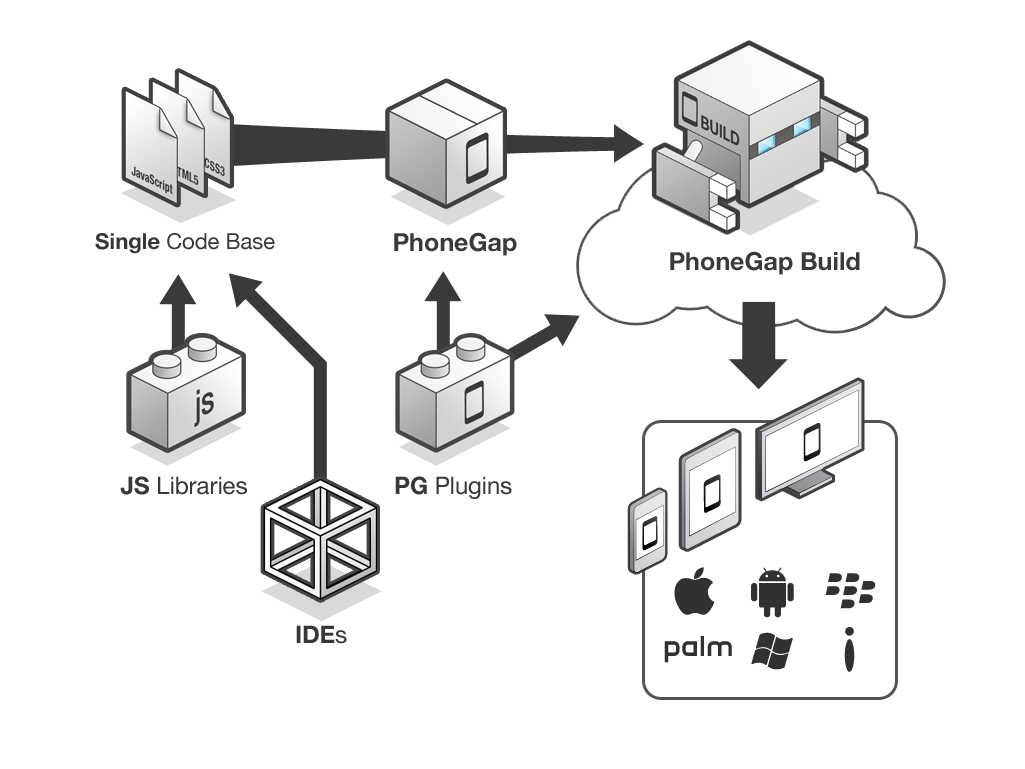
\includegraphics[width=.8\textwidth]{../resources/figs/cordova-architecture.png}
        \caption{The architecture of Apache Cordova/Adobe PhoneGap applications \cite{PhoneGap:Overview}.}
        \label{fig:cordova:architecture}
    \end{center}
\end{figure}

One of Cordova's goals is to promote the web as a first-class development platform. However, many mobile browser implementations are still lacking sufficient HTML5 support. Cordova solves this problem by providing HTML5 polyfills for these browsers. A polyfill is a replacement implementation for missing functionality. The API of the polyfill typically matches the official HTML5 API such that applications do not notice that the feature is missing. If the browser does have support for a particular feature, the browsers implementation is used. For example, the Cordova Storage API is a polyfill for the deprecated but often used Web SQL specification\footnote{\url{http://dev.w3.org/html5/webdatabase/}} and Web Storage specification\footnote{\url{http://dev.w3.org/html5/webstorage/}}. 

Cordova has a pluggable architecture, i.e. within Cordova, every device API is implemented as a plugin. This allows to (1) leave out unused device API's, reducing the size of the compiled application, and (2) create your own custom plugin. Every plugin comprises of a piece of JavaScript code and a piece of native code. Calls to the JavaScript API are marshaled and sent to the native counterpart where the request gets unmarshaled and executed. Additionally, a response is be sent back to the caller.

A comprehensive list of Cordova plugins is available online\footnote{\url{https://github.com/phonegap/phonegap-plugins}}. However, at the time of writing, there is no package manager available for Cordova plugins, like NPM\footnote{NPM is the Node Package Manager, \url{http://npmjs.org}}.

\subsection{Related projects}

There are a number of projects related to Apache Cordova that are useful when developing mobile web applications with Cordova.

\subsubsection{WEINRE}

WEINRE\footnote{\url{http://people.apache.org/~pmuellr/weinre/docs/latest/}} is part of Apache Cordova and is an acronym for ``WEb INspector REmote''. It provides access to a fully functional WebKit inspector of remote browsers. The service runs on a node\footnote{Server-side JavaScript, \url{http://nodejs.org}} server. The only requirement is to include a javascript file in the application's HTML file. When the browser starts executing the JavaScript file, it makes a persistent connection with a server through a web socket. This connection is then used for all communication between the web application and the WebKit inspector. This allows developers to inspect the DOM, resources, and run custom JavaScript commands remotely. A hosted version is available online\footnote{\url{http://debug.phonegap.com}}.

\subsubsection{Apache Ripple}

Apache Ripple\footnote{\url{http://ripple.incubator.apache.org}} is a web-based mobile environment simulator and is available as a Chrome extension. It exposes the Apache Cordova device API's and allows developers to simulate various device features in a desktop browser. For instance, you can shake the device, set a location and heading, emulate disruptive networking, etc.

\subsubsection{Adobe PhoneGap Build}

Adobe PhoneGap Build\footnote{\url{http://build.phonegap.com}}, part of Adobe Edge Tools \& Services, is an online build service for packaging Cordova/PhoneGap applications. Upon request, the application's source code is pulled from a git\footnote{Git is a popular version control system, \url{http://git-scm.org}} repository and the packaged app can be downloaded straight from the web interface. An API is available to automate the process. The service supports Android, iOS, Windows Phone, BlackBerry, WebOS, and Symbian.

Both free and paid plans (with a monthly subscription fee) are available. The free plan is entitled to only one private project, a paid plan is entitled to 25 or more private apps.

\subsubsection{Edge Inspect}

Another Adobe product is called Edge Inspect\footnote{\url{http://html.adobe.com/edge/inspect/}}, which is also part of Adobe Edge Tools \& Services. It comprises of a desktop application, a Chrome plugin and a couple of native applications and allows developers to preview web designs on multiple displays at a time. When the plugin is activated, all connected devices instantly load the same web page. At the same time, developers get access to a WebKit inspector, showing the code of any remote browser (this is actually based on WEINRE). The application also allows the developer to take screen shots the web pages displayed in a particular browser.

\subsection{Implementation of the proof-of-concept application}

The proof-of concept application is implemented as a single-page application. This eliminates page loads and thus improves overall performance of the application. The application code is all wrapped inside the native shell.  The application logic is built with AngularJS, the user interface is built on top of Bootstrap. The development workflow is based on Yeoman, which provides useful tools for scaffolding, building, previewing, testing, etc. Unit and integration tests are created with the Jasmine test framework and run with the Karma test runner. The exact role of each tool is discussed in the following sections.

\subsubsection{AngularJS}

AngularJS\footnote{\url{http://angularjs.org}} is an JavaScript MVC application framework, developed at Google. With AngularJS, developers can use a declarative programming style rather than an imperative style. This is achieved through additional HTML elements and attributes, which serve as annotations. In addition, the imperative programming style is still available to program controller code. AngularJS also provides a dependency injection system which makes testing easier. For instance, components that require user interaction or are not useful in a testing environment. Using dependency injection, they can be replaced easily with a mock. A mock is a replacement component that mimics the behaviour of the element it replaces but it does not rely on components that are not available in a testing environment.

AngularJS has proven useful from the start. The project came to live at Google because developers of the Google Feedback project were unsatisfied with the development speed. The project that already took 18 man months and 17000 lines of traditional HTML and JavaScript code, could be completely rewritten using AngularJS in three weeks by a single individual and with only 1500 lines of code \cite{Green:2013}.

\subsubsection{Bootstrap 3}

Bootstrap\footnote{\url{http://getbootstrap.com}} is a popular HTML user interface framework that came to life at Twitter. The latest revision, (version 3, still in beta) is a complete overhaul of the project, introducing a mobile-first approach. Instead of scaling down desktop pages, the new version starts from the mobile interface and scales up as the screen size increases. 

\subsubsection{Yeoman}

Yeoman\footnote{\url{http://yeoman.io}} is a collection of tools and best practices to make web development easier. It is comprised of the following tools:
\begin{itemize}
    \item \textbf{Yo} is a command-line tool used for scaffolding application code. A Yo plugin for AngularJS projects is available online\footnote{\url{https://github.com/yeoman/generator-angular}} and can generate various application artifacts like a basic project setup, controllers, services, directives, etc.
    \item \textbf{Grunt} is a command-line tool, similar to the make program\footnote{\url{https://www.gnu.org/software/make/}}. It can run various predefined JavaScript tasks: compiling LESS files, minifying javascript and CSS, linting Javascript, running unit tests, etc.
    \item \textbf{Bower} is a package manager for web applications and takes care of tracking complex dependency graphs in a project. It is available as a command line tool.
\end{itemize}

\subsubsection{Jasmine \& Karma}

One of AngularJS' focal points is writing testable code. The community has created a test runner, called Karma\footnote{\url{http://karma-runner.github.io/}}. Running Karma will start a basic server, open a collection of browser windows (even mobile browser on connected devices or a headless browser like PhantomJS\footnote{\url{http://phantomjs.org/}}) and run all the tests in these browsers. The results of the tests are then passed back to the test runner in order to report them to the user. 

The tests are coded with the Jasmine\footnote{\url{http://pivotal.github.io/jasmine/}} testing framework.

\section{Motorola Rhodes}

\subsection{General information \& history}

Rhodes\footnote{\url{http://docs.rhomobile.com}} was developed and released in 2008 by an American company called RhoMobile. Their goal was to enable developers to quickly create native applications for all smartphones. Rhodes applications make use of synchronized local data and take advantage of the device's hardware. With a local synchronization engine, called RhoSync, the emphasis is clearly on data-driven enterprise applications.

In July 2011, Motorola Solutions (the non-mobile, enterprise and government-oriented division, not the division that was acquired by Google) acquired RhoMobile. After the acquisition, Motorola introduced the commercial product RhoElements: a set of specialized features like a barcode scanner, NFC and signature capture. About one year after the acquisition, Motorola removed a lot of the features from the Rhodes framework and included them in RhoElements version 2.

The Rhodes framework is open source and freely available under the MIT license. Based on the statistics of the RhoMobile Google groups page,  community activity has significantly decreased in the last year from 722 monthly posts in June 2012 to 102 monthly posts in April 2013. However, based on the contribution history on GitHub, development activity seems to have increased since January 2013.

Rhodes currently supports all major platforms, including Android (2.1 and up), iOS (3.0 and up), Windows Phone 8 and BlackBerry (4, 5, 6 and 7).

\subsection{Architecture}

Rhodes is a cross-platform tool that creates applications that are both interpreted and hybrid at the same time. A Rhodes application is a mobile web application that runs locally on top of a Ruby web server, i.e. the application code it written in Ruby, the view is written in HTML. The architecture is depicted in \fref{fig:rhodes-architecture}.

\begin{figure}[h]
    \begin{center}
        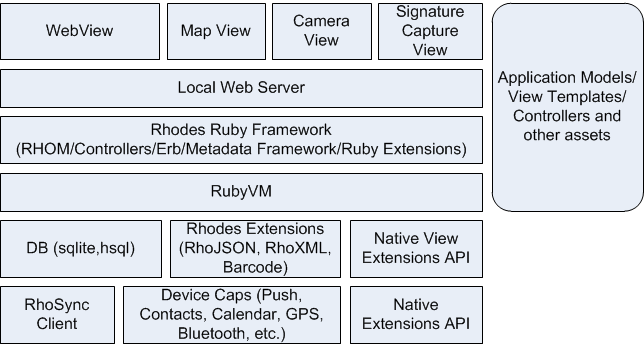
\includegraphics[width=0.9\textwidth]{../resources/figs/rhodes-architecture.png}
        \caption{The architecture of Rhodes applications \cite{Rhodes:Overview}}
        \label{fig:rhodes-architecture}
    \end{center}
\end{figure}

Rhodes also has a plugin system that allows developers to create native extensions for missing functionality. A plugin consists of a shared Ruby interface definition and native implementations for the supported platforms.

\subsection{Related projects}

Rhodes is an open-source framework is part of a collection of software, called RhoMobile Suite, which also contains other software products that fit strategically in this suite. These products are discussed briefly in this section.

\subsubsection{RhoElements}

RhoElements is a commercial product in the RhoMobile Suite and therefore requires a license. It contains a substantial amount of additional functionality that is useful for enterprise applications like NFC, barcode readers, etc. This functionality was removed from Rhodes in version 3.3.3.

\subsubsection{RhoConnect}

RhoConnect is an open-source product in the RhoMobile Suite and serves as a mobile orchestrator. It takes care of data synchronization between backend applications and mobile devices. The libraries for this integration are already available in the Rhodes framework.

\subsubsection{RhoHub}

RhoHub\footnote{\url{https://app.rhohub.com/}} is a cloud platform that developers can use to host and build their applications. Developers can push their code to a private git repository from which the application can be built for Android, iOS, BlackBerry, Windows Mobile, and Windows.

\subsubsection{RhoStudio}

RhoStudio is an Ruby IDE, based on Eclipse 3.7, and contains a custom plugin for Rhodes and RhoElements application development. It is freely available as part of the RhoMobile Suite.

\subsection{Implementation of the proof-of-concept application}

The proof-of concept application is implemented as a multi-page application because it is the way Rhodes is intended to be used. The downside of this approach is it introduces waiting time for every page it loads. The user interface is also based on Bootstrap.

The development of the proof-of-concept application was aborted early because the tooling was bugged and the performance of the resulting Rhodes applications was unsatisfying. On an entry-level smartphone, loading a page took 30 seconds and on a high-end smartphone page loads still take 7 seconds. Capgemini deemed this unacceptable and Rhodes was no longer considered a viable alternative.